\section*{Příloha A: Ukázka softwarového MATLAB řešení}
\label{att:sw_matlab}
\addcontentsline{toc}{section}{Příloha A: Ukázka softwarového MATLAB řešení}

\begin{figure}[H]
    \begin{center}
        \textcolor{cyan}{\fboxrule=0.3pt\fboxsep=0pt\fbox{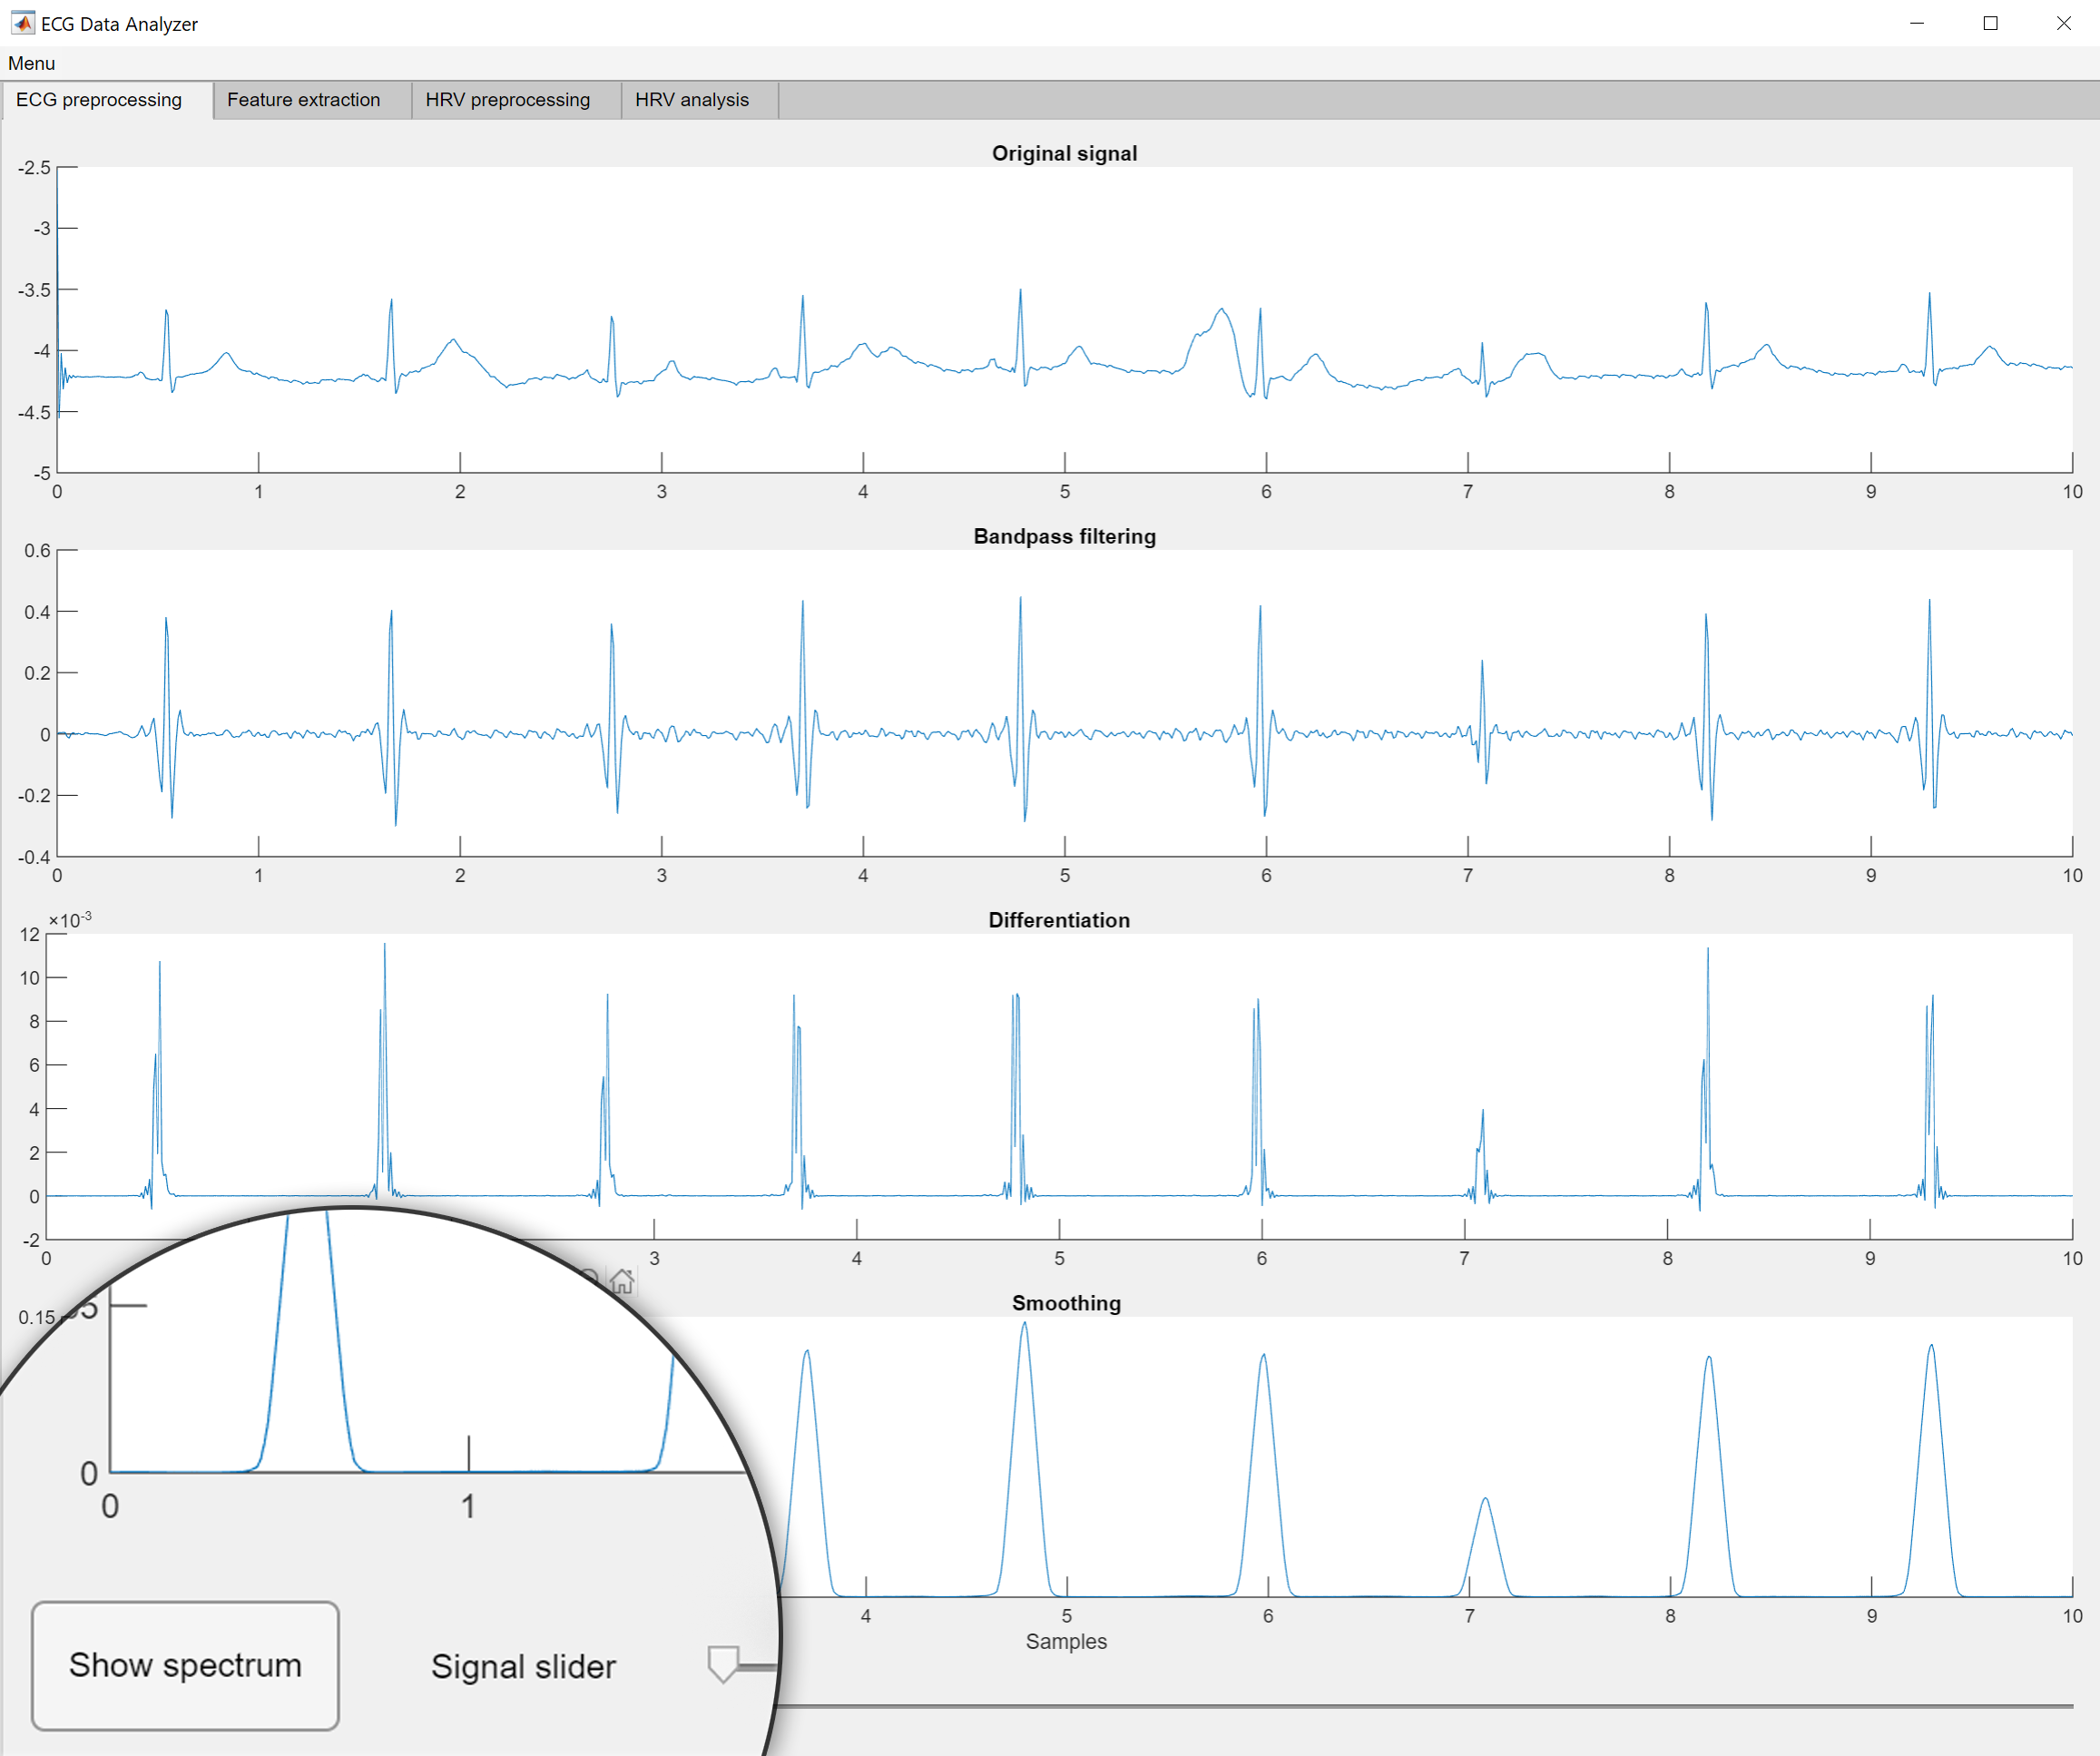
\includegraphics[width=0.8\textwidth]{matlab_EDA/tab1}}}
        \caption{Hlavní okno aplikace -- karta ECG preprocessing}
        \label{fig:results_matlab_tab1}
    \end{center}
\end{figure}

\begin{figure}[H]
    \begin{center}
        \textcolor{cyan}{\fboxrule=0.3pt\fboxsep=0pt\fbox{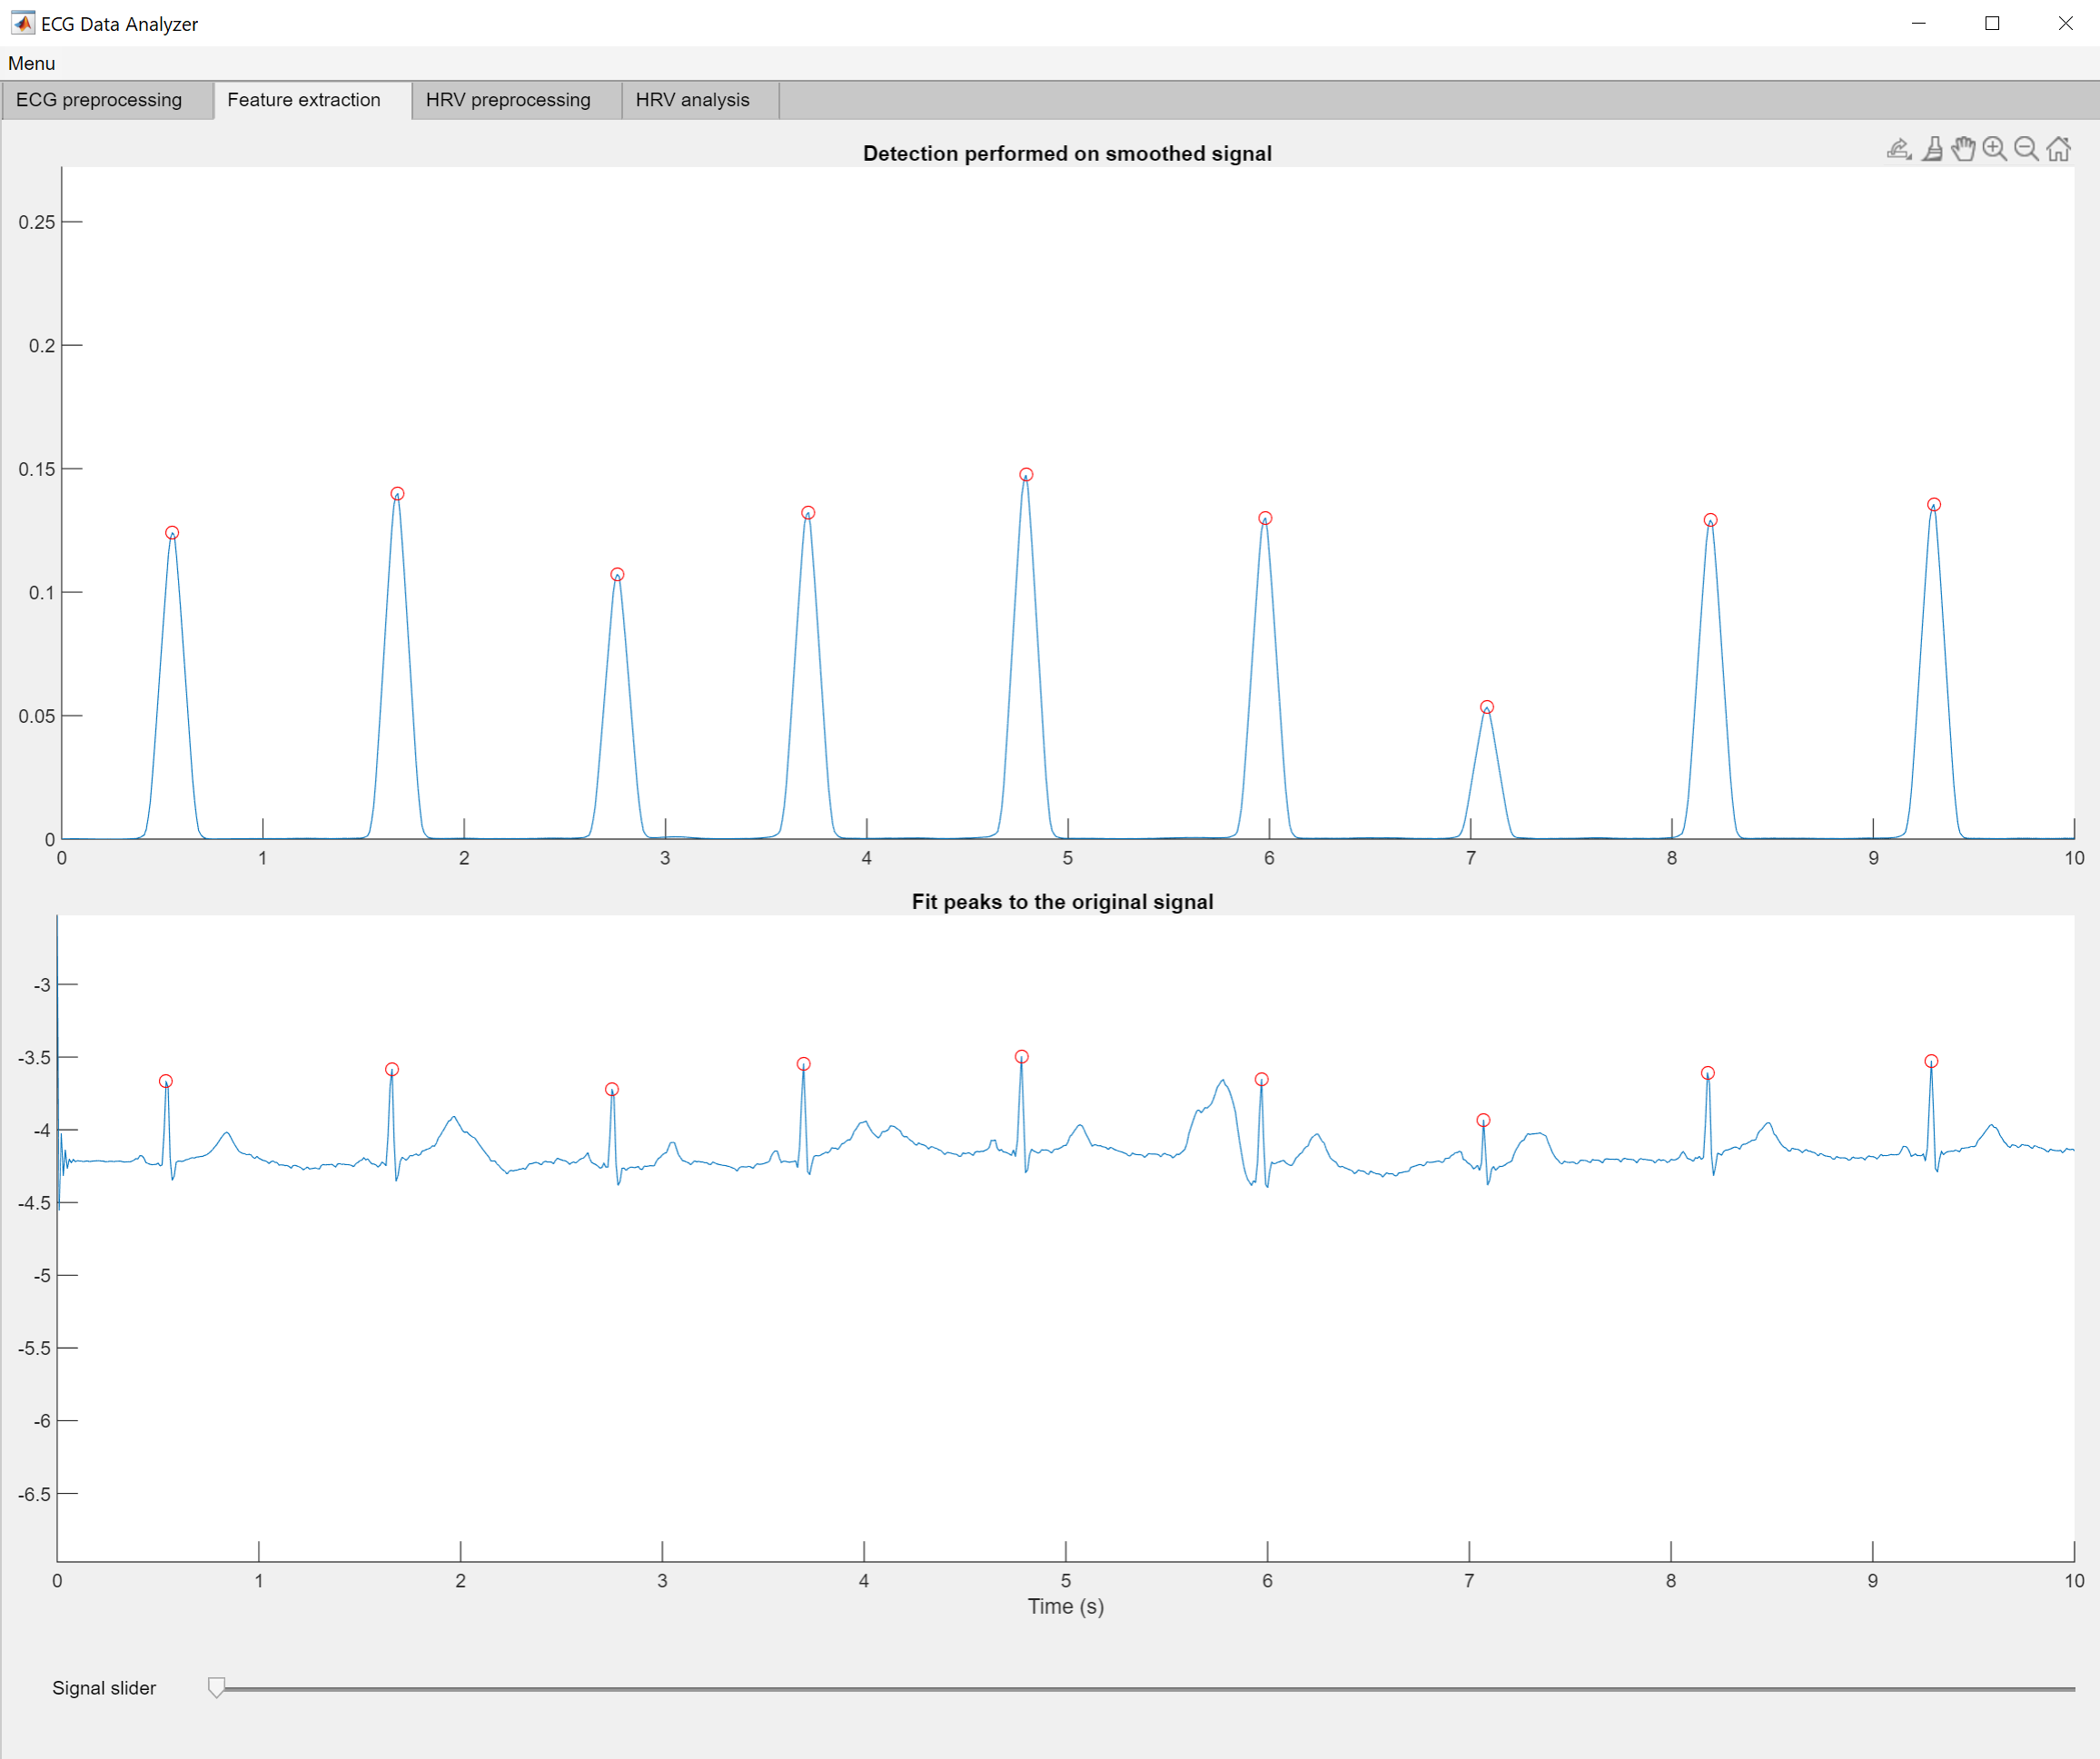
\includegraphics[width=0.8\textwidth]{matlab_EDA/tab2}}}
        \caption{Hlavní okno aplikace -- karta Feature extraction}
        \label{fig:results_matlab_tab2}
    \end{center}
\end{figure}

\begin{figure}[H]
    \begin{center}
        \textcolor{cyan}{\fboxrule=0.3pt\fboxsep=0pt\fbox{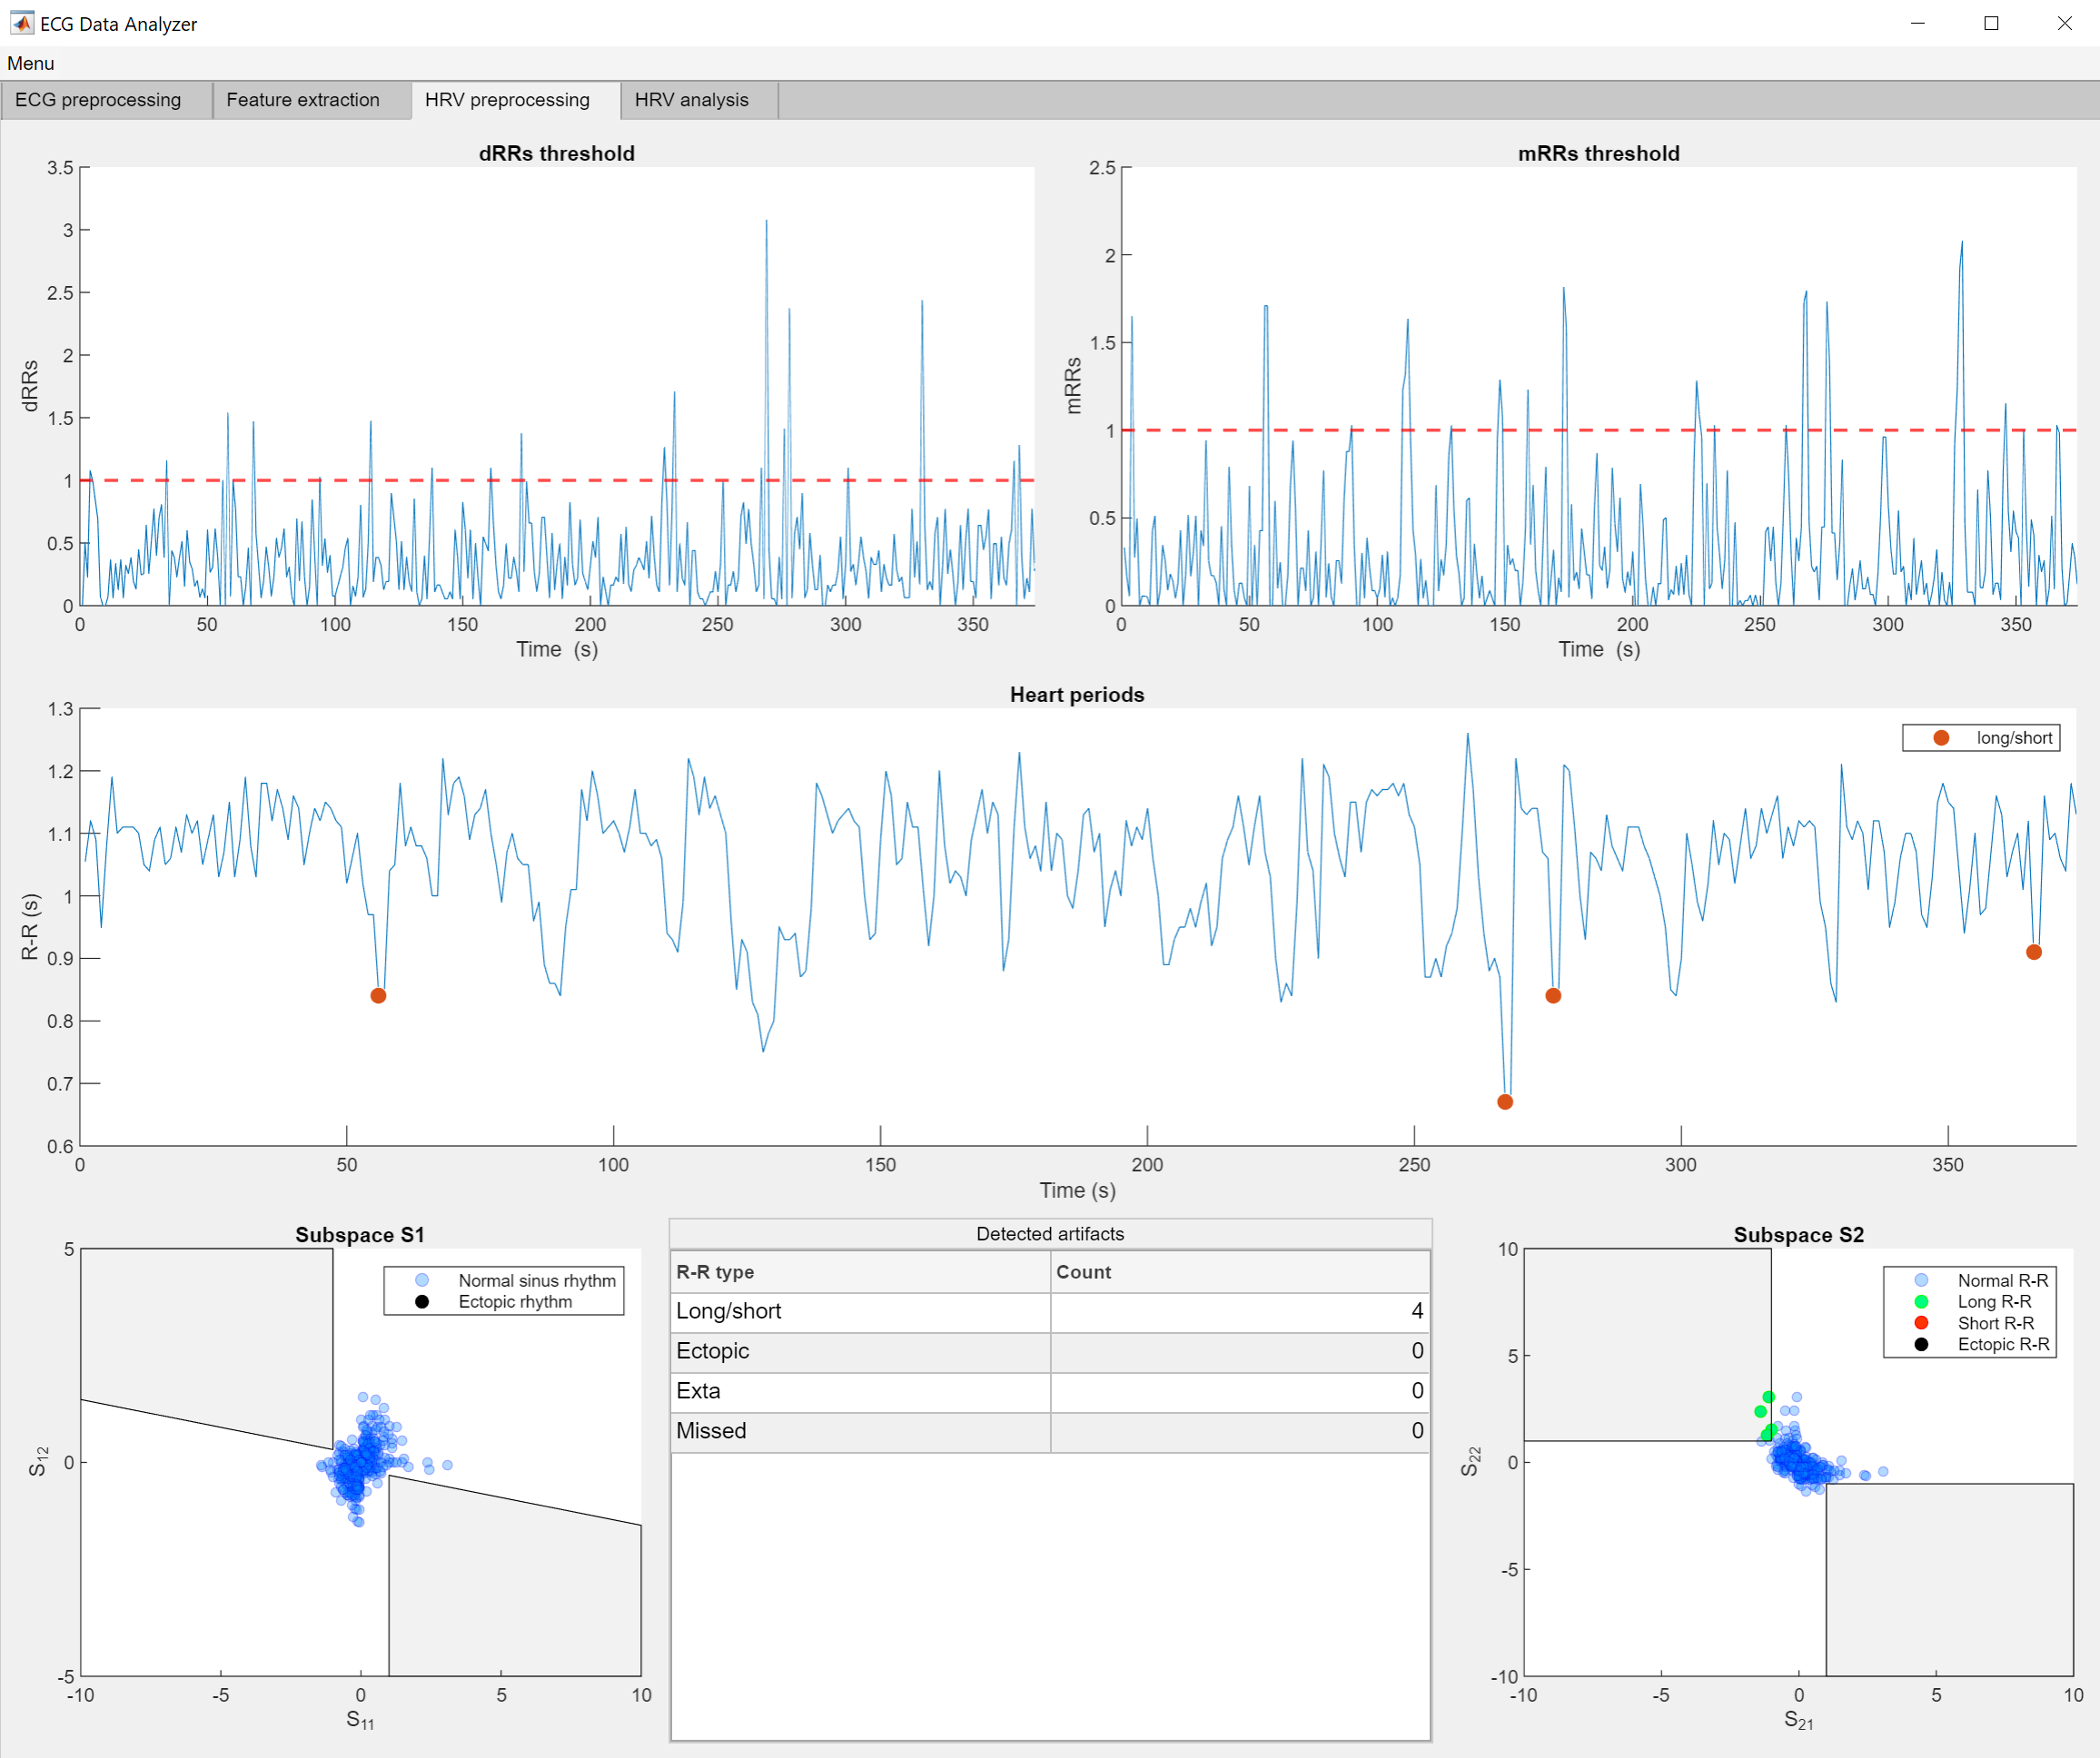
\includegraphics[width=0.8\textwidth]{matlab_EDA/tab3}}}
        \caption{Hlavní okno aplikace -- HRV preprocessing}
        \label{fig:results_matlab_tab3}
    \end{center}
\end{figure}

\begin{figure}[H]
    \begin{center}
        \textcolor{cyan}{\fboxrule=0.3pt\fboxsep=0pt\fbox{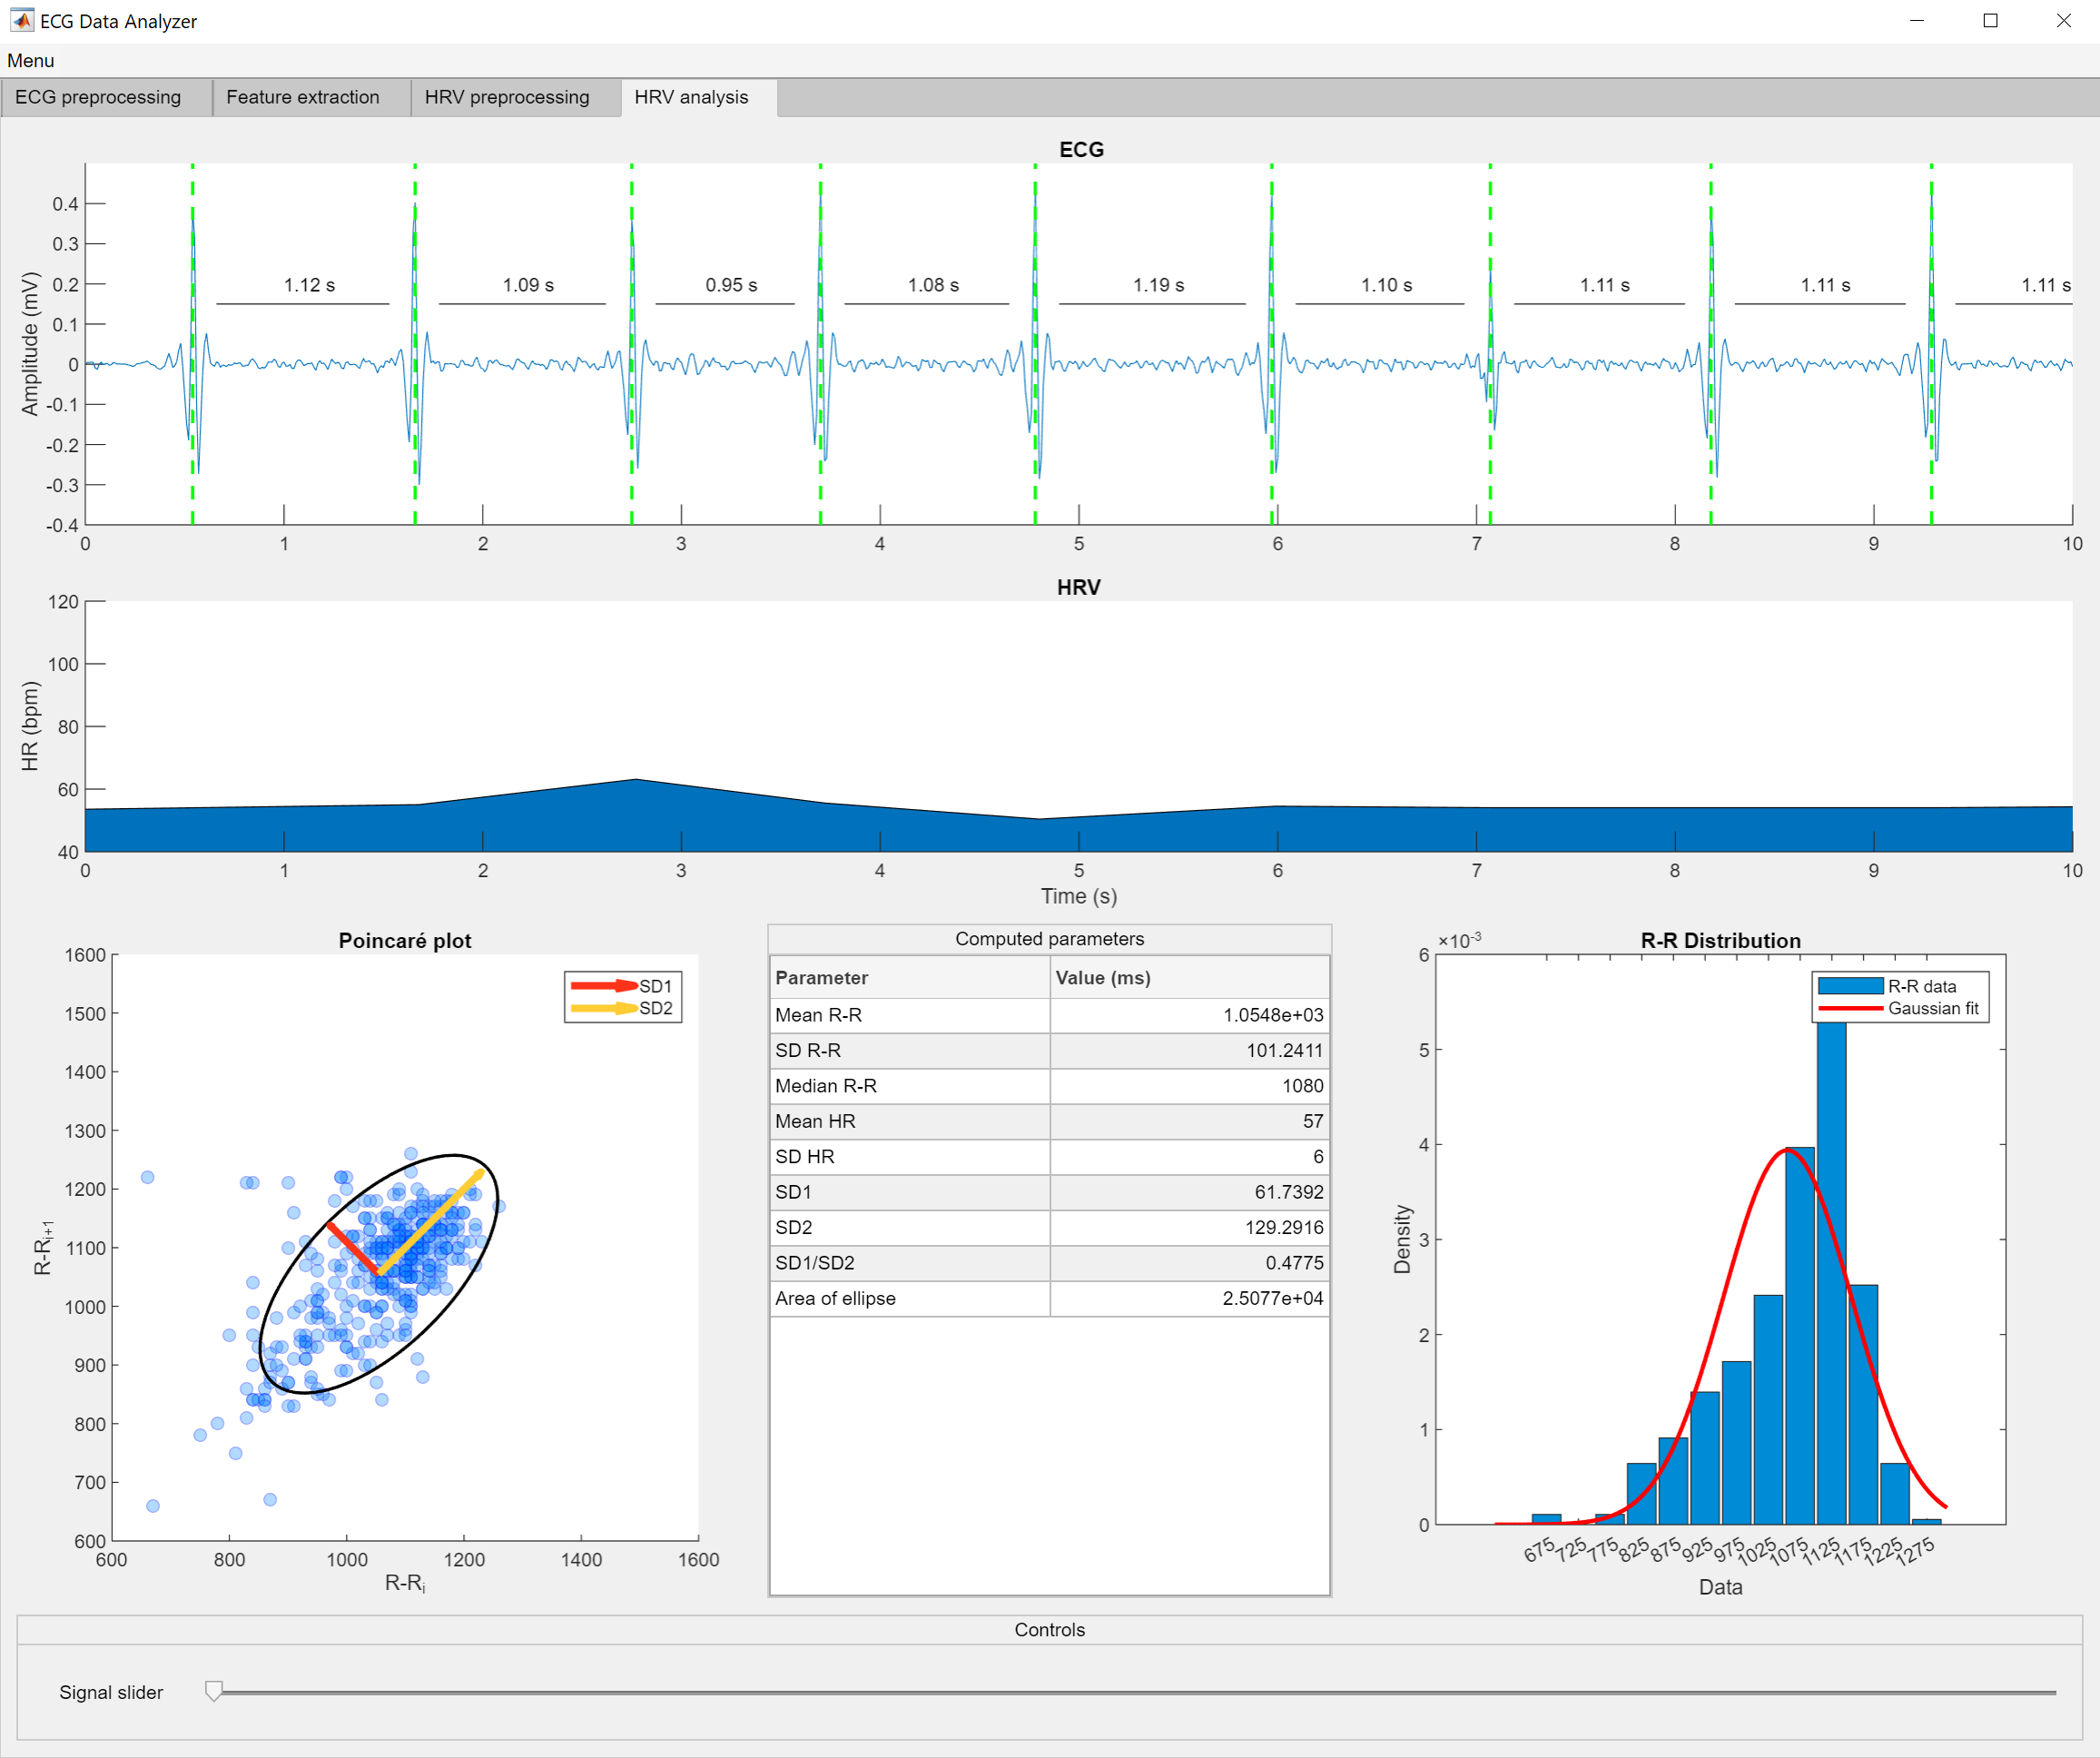
\includegraphics[width=0.8\textwidth]{matlab_EDA/_tab4}}}
        \caption{Hlavní okno aplikace -- karta HRV analysis}
        \label{fig:results_matlab_tab4_}
    \end{center}
\end{figure}

\clearpage

%\section*{Příloha B: Informovaný souhlas a stanovisko etické komise}
%\label{app:typo}
%\addcontentsline{toc}{section}{Příloha B: Základní typografické zásady}

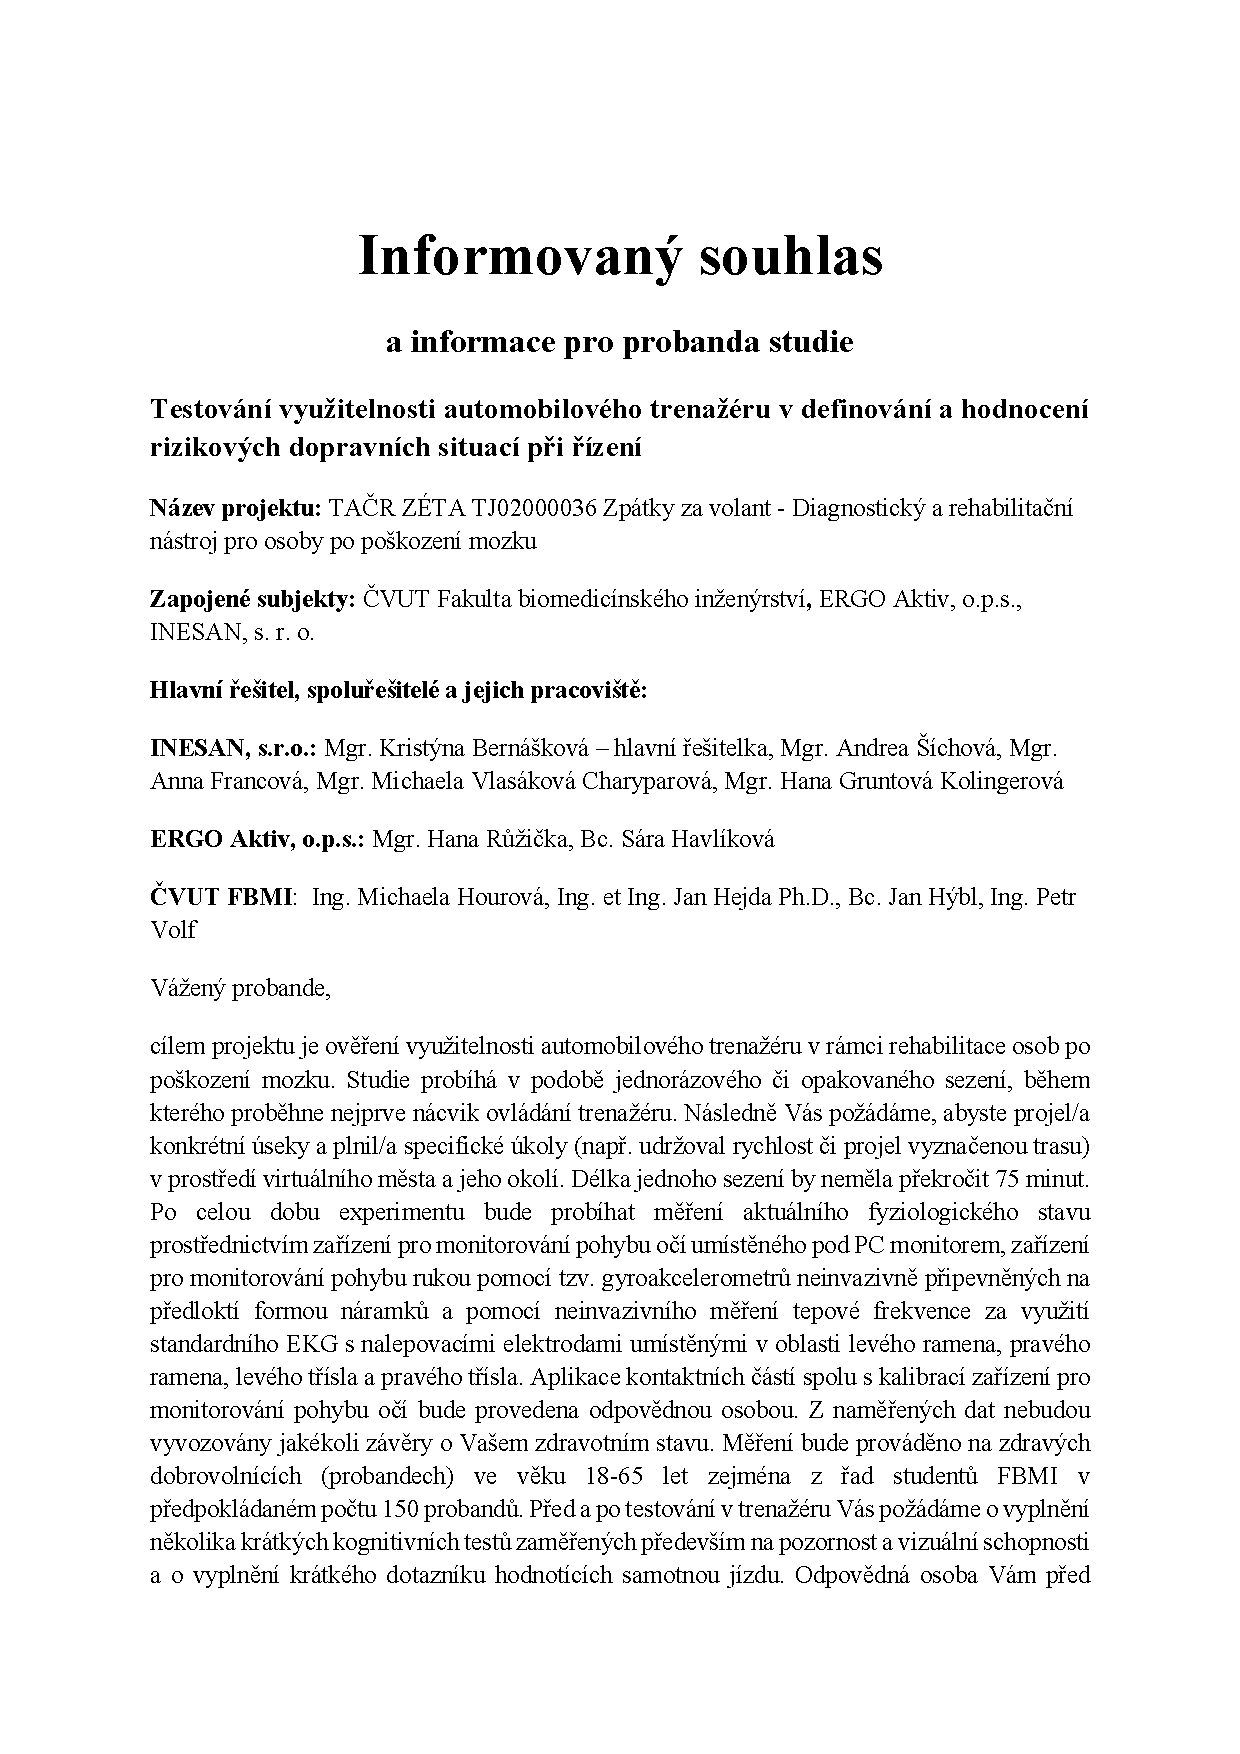
\includepdf[pages=1,pagecommand={\section*{Příloha B: Informovaný souhlas a stanovisko etické komise}\addcontentsline{toc}{section}{Příloha B: Informovaný souhlas a stanovisko etické komise}\label{pdf:souhlas}}]{informovany_souhlas}
\includepdf[pages=2-,pagecommand={}]{informovany_souhlas}

\clearpage


\includepdf[pages=1,scale=0.8,pagecommand={}]{potvrzena_zadost_eticke_komise.pdf}

\clearpage

\section*{Příloha C: Výsledné Poicarého grafy}
\label{att:poincare_plots}
\addcontentsline{toc}{section}{Příloha C: Výsledné Poicarého grafy}

\begin{figure}[H]
    \centering
    \begin{subfigure}{0.45\textwidth}
        \centering
        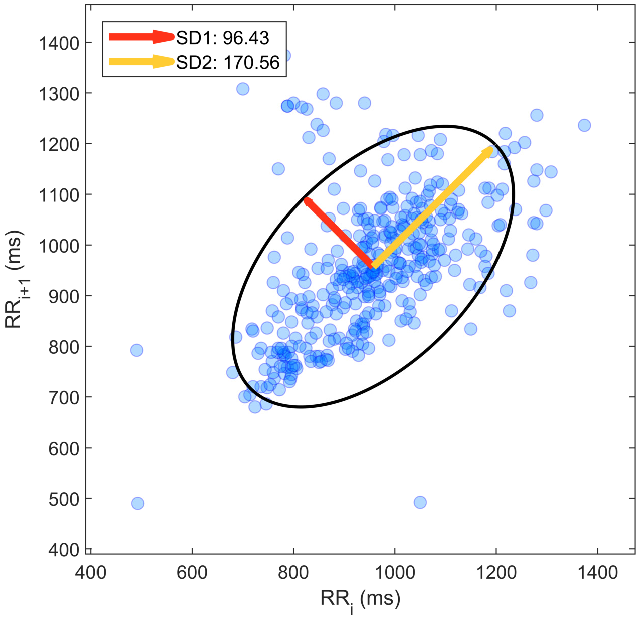
\includegraphics[width=1\linewidth]{figures/pp/rest_1}
        \caption{Proband 1 -- V klidu}
    \end{subfigure}
    \hspace{12pt}
    \begin{subfigure}{0.45\textwidth}
        \centering
        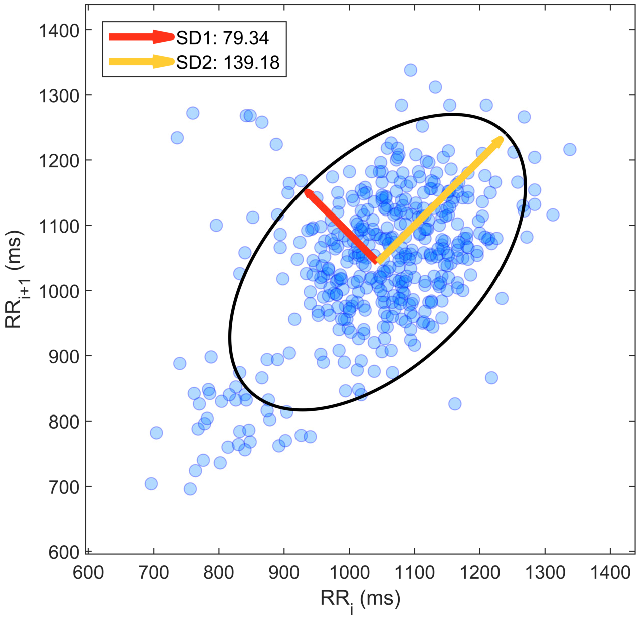
\includegraphics[width=1\linewidth]{figures/pp/stroop_1}
        \caption{Proband 1 -- Kognitivní zátěž}
    \end{subfigure}
    \par\bigskip
    \begin{subfigure}{0.45\textwidth}
        \centering
        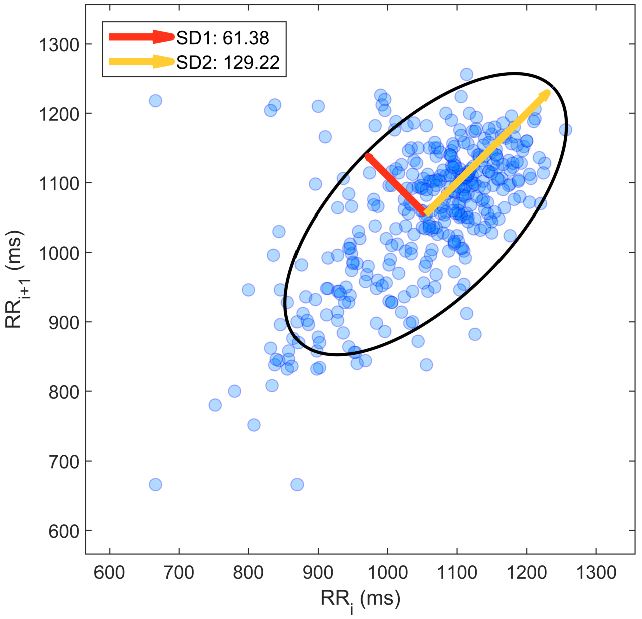
\includegraphics[width=1\linewidth]{figures/pp/rest_2}
        \caption{Proband 2 -- V klidu}
    \end{subfigure}
    \hspace{12pt}
    \begin{subfigure}{0.45\textwidth}
        \centering
        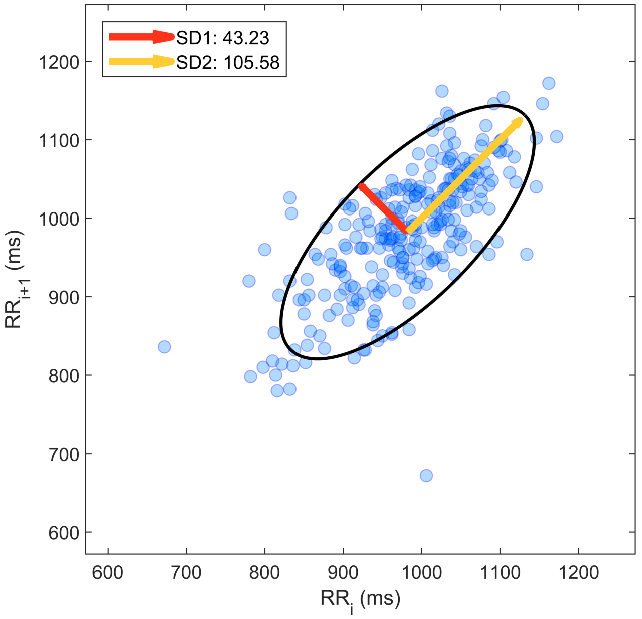
\includegraphics[width=1\linewidth]{figures/pp/stroop_2}
        \caption{Proband 2 -- Kognitivní zátěž}
    \end{subfigure}
    \par\bigskip
    \begin{subfigure}{0.45\textwidth}
        \centering
        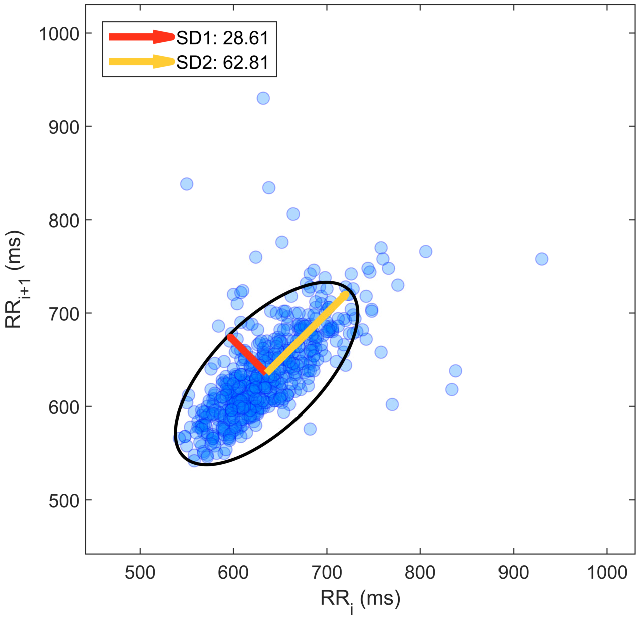
\includegraphics[width=1\linewidth]{figures/pp/rest_3}
        \caption{Proband 3 -- V klidu}
    \end{subfigure}
    \hspace{12pt}
    \begin{subfigure}{0.45\textwidth}
        \centering
        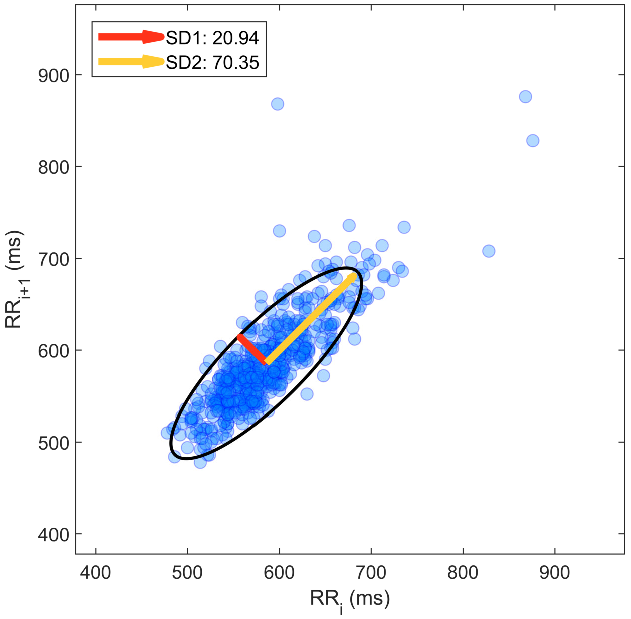
\includegraphics[width=1\linewidth]{figures/pp/stroop_3}
        \caption{Proband 3 -- Kognitivní zátěž}
    \end{subfigure}
\end{figure}
\begin{figure}[H]\ContinuedFloat 
    \centering
    \begin{subfigure}{0.45\textwidth}
        \centering
        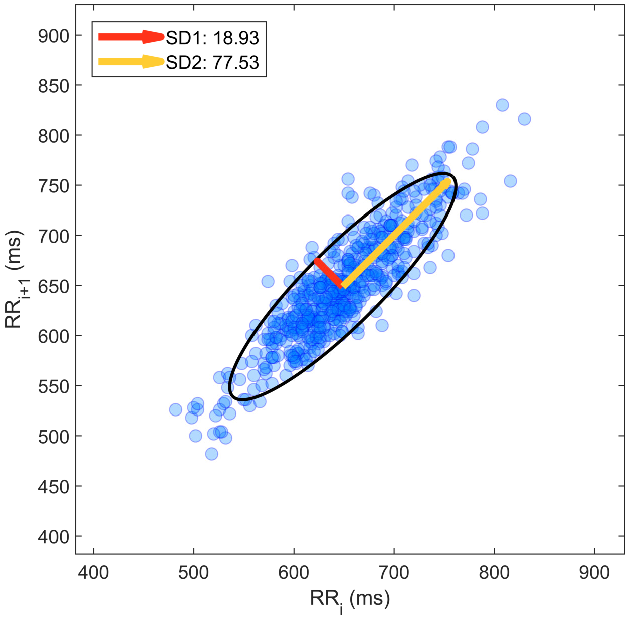
\includegraphics[width=1\linewidth]{figures/pp/rest_4}
        \caption{Proband 4 -- V klidu}
    \end{subfigure}
    \hspace{12pt}
    \begin{subfigure}{0.45\textwidth}
        \centering
        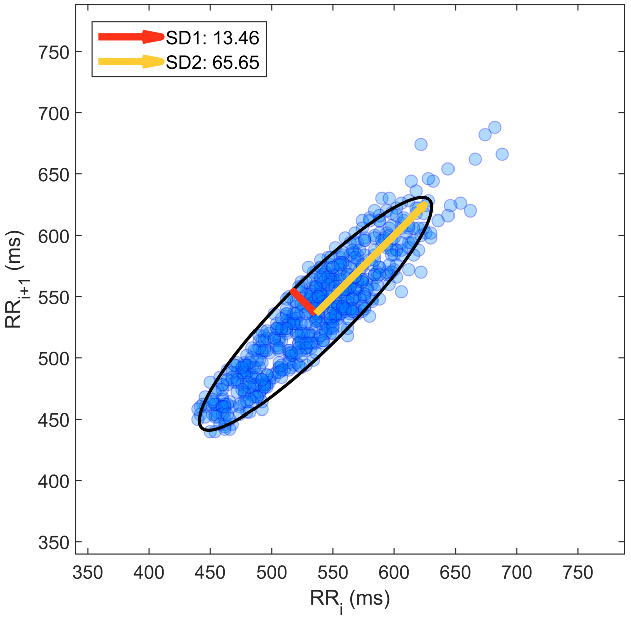
\includegraphics[width=1\linewidth]{figures/pp/stroop_4}
        \caption{Proband 4 -- Kognitivní zátěž}
    \end{subfigure}
    \par\bigskip
    \begin{subfigure}{0.45\textwidth}
        \centering
        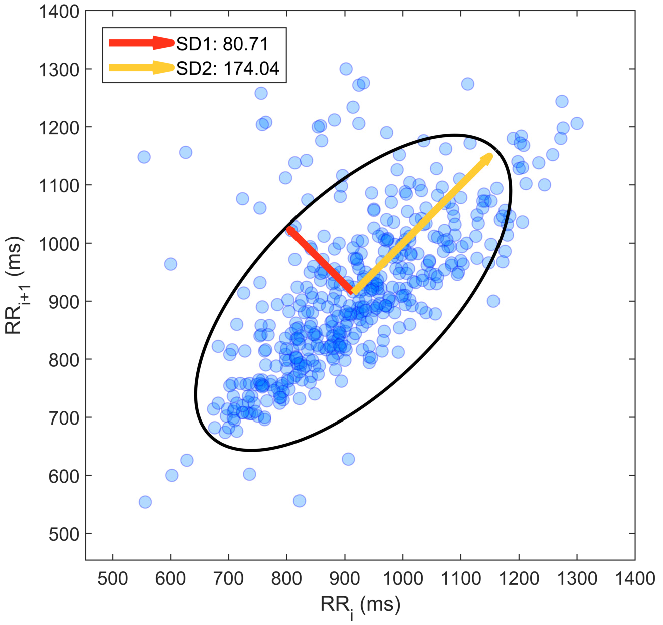
\includegraphics[width=1\linewidth]{figures/pp/rest_5}
        \caption{Proband 5 -- V klidu}
    \end{subfigure}
    \hspace{12pt}
    \begin{subfigure}{0.45\textwidth}
        \centering
        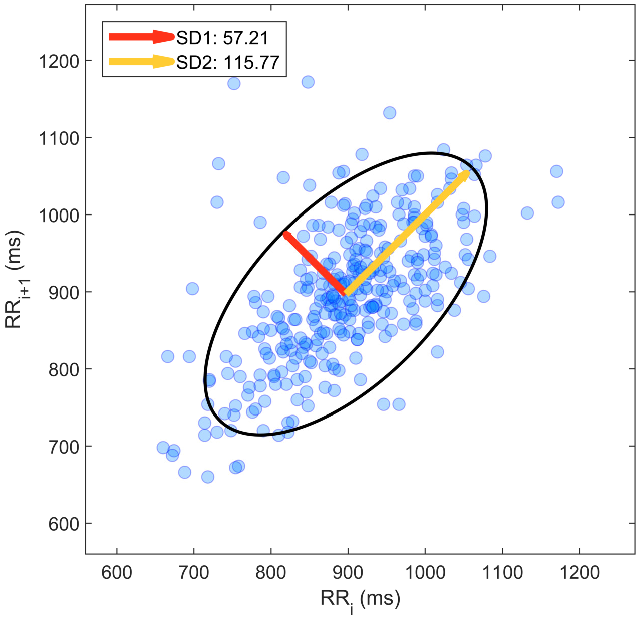
\includegraphics[width=1\linewidth]{figures/pp/stroop_5}
        \caption{Proband 5 -- Kognitivní zátěž}
    \end{subfigure}
    \caption{Výsledné Poincarého grafy pro úseky v klidu a při stimulaci kognitivní zátěže}
    \label{fig:attachment_poincares_plots}
\end{figure}

\clearpage

\section*{Příloha D: Obsah přiloženého CD/DVD}
\label{att:data}
\addcontentsline{toc}{section}{Příloha D: Obsah přiloženého CD/DVD}

\begin{figure}[h]
    \begin{minipage}{0.95\textwidth}
        \dirtree{%
            .1 /.
            .2 src.
            .3 BBPM\DTcomment{Zdrojový kód Python aplikace \textit{BBPM}}.
            .3 reports\DTcomment{Reporty z aplikace \textit{Kubios HRV Standard}}.
            .3 thesis\DTcomment{Zdrojový kód bakalářské práce ve formátu \LaTeX{}}.
            .3 QRSDetectors\DTcomment{MATLAB implementace QRS detektorů}.
            .4 pan\_tompkins.m.
            .4 hamilton\_tompkins.m.
            .4 nabian.m.
            .3 data.mat\DTcomment{Naměřená a zpracovaná data}.
            .3 ECGDataAnalyzer.mlapp\DTcomment{Navržená MATLAB aplikace}.
            .3 filters.m\DTcomment{Navržené digitální filtry}.
            .3 statistics.m\DTcomment{Statistické zpracování dat}.
            .3 swtest.m\DTcomment{Shapiro-Wilkův test normality}.
            .2 text.
            .3 abstract\_cs.txt\DTcomment{Abstrakt česky}.
            .3 abstract\_en.txt\DTcomment{Abstrakt anglicky}.
            .3 keywords\_cs.txt\DTcomment{Klíčova slova v ČJ}.
            .3 keywords\_en.txt\DTcomment{Klíčova slova v AJ}.
            .3 assignment.pdf\DTcomment{Zadání bakalářské práce v PDF}.
            .3 17PBBBP\_483417\_Marek\_Sokol.pdf\DTcomment{Bakalářská práce v PDF}.
        }
    \end{minipage}
\end{figure}

